\chapter{Visibility-Weighted Saliency for Volume Visualization \label{visibility-weighted_saliency}}
%Volume visualization has been widely used to depict complicated 3D structures in volume data sets.
%However, obtaining clear visualization of the features of interest in a volume is still a major challenge.
In volume visualization, the clarity of features depends on the transfer function, the viewpoint and spatial distribution of features in the volume data set.
In this chapter, we propose visibility-weighted saliency as a measure of visual saliency of features in volume rendered images, in order to assist users in choosing suitable viewpoints and designing effective transfer functions to visualize the features of interest. Visibility-weighted saliency is based on a computational measure of perceptual importance of voxels and the visibility of features in volume rendered images.
The effectiveness of this scheme is demonstrated by test results on two volume data sets.

%-------------------------------------------------------------------------
\section{Introduction}
Volume visualization is an active branch of scientific visualization. It is a method of extracting meaningful information from volumetric data sets, which usually contain complex structures of various material.
First introduced by Levoy \cite{levoy_display_1988} for visualization of volume data, volume visualization has been widely used in various sciences to create insightful visualizations from both simulated and measured data.

A crucial step in volume visualization is transfer function specification. Transfer functions assign visual properties, including color and opacity, to the volume data being visualized. Hence, transfer functions determine which structures will be visible and how they will be rendered.
An appropriate transfer function can quickly reveal large amounts of information of the data set to the viewer.
However, obtaining an effective transfer function is a non-trivial task, which involves a significant amount of tweaking of color and opacity.
A cause of this problem is the lack of an objective measure to quantify the quality of transfer functions \cite{correa_visibility_2011}.

Although user studies are useful in evaluating some fundamental characteristics of visualization techniques, it is not possible to conduct a user study for each individual visualization every time it is created.
Several computational measures of visual saliency that model human attention have been developed \cite{itti_model_1998} \cite{harel_graph-based_2006}.
Kim and Varshney \cite{kim_saliency-guided_2006} introduced the saliency field, which measures visual saliency of voxels using the center-surround operator based on the difference of Gaussian-weighted averages at a fine and a coarse scale.
However, salient voxels may be occluded by other voxels close to the viewer in certain viewpoints and thus these salient voxels become invisible in the volume rendered image. In order to measure the visual saliency of features in volume rendered images, it is necessary to consider both the saliency and the visibility of the voxels which form the feature.

In this chapter, we propose visibility-weighted saliency as an improved measure of the visual saliency of features in volume rendered images. Visibility-weighted saliency is a combination of feature visibility \cite{wang_efficient_2011} and saliency fields \cite{kim_saliency-guided_2006}.
Feature visibility measures the contribution of each feature to the volume rendered image and saliency fields measure
%the visual saliency of each voxel in its local neighborhood.
how strongly each voxel stands out in its local neighborhood.
The visibility-weighted saliency are presented in two different ways, i.e. visibility-weighted saliency fields and feature saliency histograms. Visibility-weighted saliency fields display the spatial distribution of visual saliency of features and feature saliency histograms provide quantitative information about the perceptual importance of the features.
With visibility-weighted saliency, the saliency of features rendered in different viewpoints with different transfer functions can be measured in a quantitative and fully automated way.
Thus, this technique can be used to guide users in choosing appropriate viewpoints and designing effective transfer functions for the features of interest in volume visualization.
This technique is also useful for understanding how much different parts of the volume contribute to the final image and how different tissues occlude each other and interfere with each other's visibility.

%-------------------------------------------------------------------------
\section{Related Work}
Several computational models of visual saliency for modeling human attention have been developed.
Itti et al. \cite{itti_model_1998} developed a computational model of visual attention based on the center-surround operators in an image. This center-surround mechanism has the intuitive appeal of being able to identify regions that are different from their surrounding context.
Lee et al. \cite{lee_mesh_2005} proposed saliency for meshes based on a multi-scale center-surround mechanism that operates on local curvature. Kim and Varshney \cite{kim_saliency-guided_2006} presented the use of a center-surround operator using the Laplacian of Gaussian-weighted averages of appearance attributes to enhance selected regions of a volume and validated their work using an eye-tracking user study. Shen et al. \cite{shen_spatiotemporal_2015} extended this technique to spatiotemporal volume saliency to detect both spatial and temporal changes.

Visibility measures the impact of individual voxels on the image generated by a volumetric object and visibility distribution can be utilized as a measure on the quality of transfer functions as users explore the transfer function space. Visibility has been studied to measure the quality of a given viewpoint \cite{bordoloi_view_2005} \cite{viola_importance-driven_2004} and to enhance the rendering process with cutaway views.
Correa and Ma \cite{correa_visibility_2011} introduced visibility histogram, which describes the accumulated visibility of each intensity value in the transfer function.

Ruiz et al. \cite{ruiz_automatic_2011} proposed an automatic method to generate a transfer function by minimizing the Kullback-Leibler divergence between the observed visibility distribution and a target distribution provided by the user. Wang et al. \cite{wang_efficient_2011} extended the idea of visibility histogram to feature visibility and introduced an interaction scheme where the opacity of each feature was generated automatically based on user-defined visibility values. Visibility distribution is also used in automating color mapping \cite{cai_automatic_2013} and 2D transfer functions \cite{qin_voxel_2015}.

%A number of general quality metrics have been proposed, including abstraction \cite{chen_measuring_2005} \cite{van_wijk_value_2005} and aesthetics \cite{filonik_measuring_2009} and visual saliency \cite{janicke_salience-based_2010}.
%Giesen et al. \cite{giesen_conjoint_2007} presented an user study design and analysis strategy geared to measure preceived quality in volume rendering.
%Wu et al. \cite{wu_quantitative_2010} described four types of quantitative assessments for volume rendered images, which are distinguishability measure, edge consistency measure, contour clarity measure and depth coherence measure.


%Various strategies have been proposed to simplify transfer function specification \cite{pfister_transfer_2001}.
%Data-centric strategies examine the properties of volume data sets.
%Overlapping intensity intervals corresponding to different materials make boundary detection difficult. Classical approaches try to detect boundary information between tissues by introducing derived attributes such as first and second derivatives to isolate materials \cite{kindlmann_semi-automatic_1998} \cite{kniss_multidimensional_2002} \cite{kindlmann_transfer_2002}.
%In this case, the transfer functions are extended to multidimensional feature spaces. As a result, the interaction of transfer functions becomes more complex and unintuitive as the dimensionality becomes higher.
%%Even two-dimensional transfer functions require a considerable amount of user interaction to find a meaningful shape \cite{arens_survey_2010}.
%Even in the case of two-dimensional transfer functions, a considerable amount of user interaction is
%required in order to come up with meaningful results \cite{arens_survey_2010}.


%Compared to visibility histograms, visibility volumes have a distinctive advantage, i.e. they maintain the spatial information of voxels in the volume.


%A number of approaches have been proposed to automate the design of transfer functions.
%Wu and Qu \cite{wu_interactive_2007} developed a method that uses editing operations and stochastic search of the transfer function parameters to maximize the similarity between volume-rendered images given by the user.
%Maciejewski et al. \cite{maciejewski_structuring_2009} described a method to structure attribute space in order to guide users to regions of interest within the transfer function histogram.
%Chan et al. \cite{chan_perception-based_2009} developed a system to optimize transparency automatically in volume rendering based on Metelli's episcotister model to improve the perceptual quality of transparent structures.
%Correa and Ma \cite{correa_visibility-driven_2009} proposed the visibility histogram to guide the transfer function design.

%-------------------------------------------------------------------------
\section{Method}
For 2D images, intensity and color are the most important attributes. In volume visualization, the intensity and color in the final images result from the blending of alpha and color determined by user-specified transfer functions in a specific viewpoint.
The saliency field is a view-independent scalar field that contains the visual saliency of each voxel in the volume data. The visual saliency of voxels represents the perceptual importance in 3D space, however it does not reflect how visible the voxels are in the final 2D images.

In order to take into account both the visual saliency of voxels in 3D space and the contribution of the voxels to the final 2D images of the rendered data set, we propose a visibility-based saliency metric, which attempts to measure the impact of individual voxels as well as user-specified features on volume rendered images.
This technique aims to assist users in gaining insight into the internal structure of the data set and understanding the contribution of different features to the final image.

%The visibility-based saliency field is based on a visibility field and a saliency field. The visibility field contains the opacity contribution of each voxel to the final 2D image and the saliency field represents the visual saliency of each voxel in the 3D volume data.

%Our method uses the center-surround mechanism to compute visual saliency of voxels. The center-surround mechanism has the intuitive appeal of being able to identify regions that are different from their surrounding context and it has been successfully applied to problems on 2D images \cite{itti_model_1998}, 3D meshes \cite{lee_mesh_2005} and 3D volumetric data \cite{kim_saliency-guided_2006}.

In this section, we describe visibility fields, saliency fields, visibility-weighted saliency fields and visibility-weighted feature saliency. In order to better illustrate the effects of these techniques, we present the results of applying these techniques to an synthetic data set from two different viewpoints in our discussion.

\subsection{Visibility Fields \label{visibility_fields}}
Direct volume rendering (e.g. ray-casting) is a technique that renders a 2D projection of the 3D volume data set. The rendering of a volume, which essentially is a block of 3D data, involves alpha blending and color composition of voxels. The resulting 2D image is acquired by blending the color and opacity of voxels along the view direction. The transfer function determines the color and opacity of individual voxels based on their data attributes such as intensity. However, the contribution of a voxel to the rendered image is determined by both the opacity of this voxel and the opacity of those voxels in front of the current voxel in the view direction.
This mechanism is described in the front-to-back compositing equations \cite{emsenhuber_visibility_2008}.
\[
C_{i}=(1-A_{i-1})c_{i}+C_{i-1}
\addtag \]
\[
A_{i}=(1-A_{i-1})a_{i}+A_{i-1}
\addtag \]
where $ a_{i} $ and $ c_{i} $ are opacity and color of voxel $ i $, and $A_{i}$ and $C_{i}$ are the accumulated opacity and color at  voxel $ i $.

Therefore, the visibility of voxel $ i $ can be calculated as
\[ v_{i}=A_{i}-A_{i-1}=(1-A_{i-1})a_{i} 
\addtag \]
and the visibility field is simply the visibility of all the voxels in the volume $ V $
\[ V=\set{v_{i}|i \in V} 
\addtag \]

The visibility field is dependent on both the viewpoint and the transfer function, therefore it can be used to analyze the visualization of the volume data. The visibility field is particularly useful for understanding what parts of the data set are being rendered and how different tissues occlude each other (Figure~\ref{fig:disks_combined}).

\begin{figure}
	\centering
	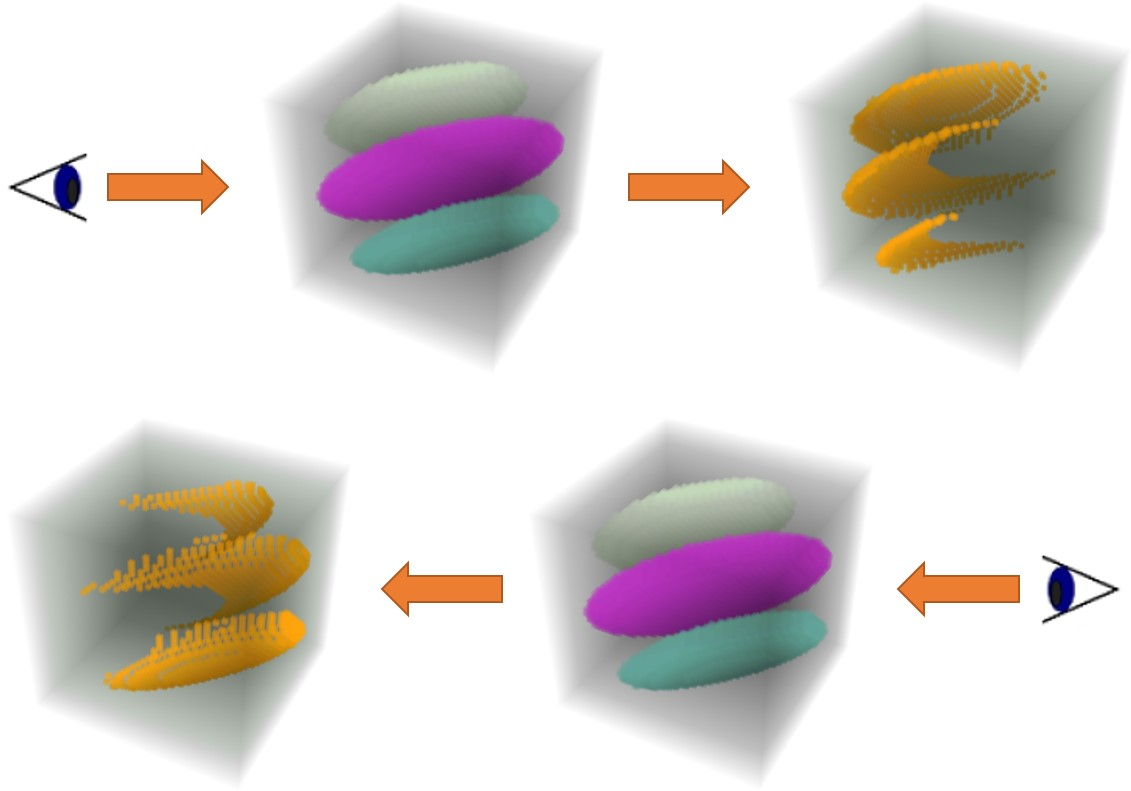
\includegraphics[width=1\linewidth]{images/disks_combined}
	\caption{A synthetic volume data set consisting of three solid disk-like features is shown. The images in the first row show the final image and the corresponding visibility field from a viewpoint on the left. The images in the second row shows the final image and visibility field from a viewpoint on the right. The visibility fields display what parts of the volume contribute most to the images and how tissues in the front occlude those in the back.}
	\label{fig:disks_combined}
\end{figure}

In terms of implementation, the computation of visibility fields can be performed in real-time on a GPU.
Correa and Ma \cite{correa_visibility_2011} employed a scattering approach for GPU-assisted computation of the visibility histogram, which scatters the pixel points to the right bin in the histogram. Wang et al. \cite{wang_efficient_2011} used the multiple rendering targets (MRT) extension of OpenGL 2.0 and above to achieve the computation of visibility for up to 32 features.
Instead of grouping visibility values into intensity bins to acquire visibility distribution over intensity ranges (histograms), we are interested in the actual spatial visibility distribution, i.e. visibility field. We perform slice-based rendering on a GPU by rendering a series of quads which are parallel to the viewing plane, one for each slice. The fragments which do not belong to the volume are discarded. Then the visibility values are computed by subtracting the accumulated opacity of the previous slice from that of the current slice. After collecting the visibility values of all voxels, the visibility field can be constructed.

\subsection{Saliency Fields \label{saliency_fields}}
Because viewers pay greater visual attention to regions that they find salient \cite{palmer_vision_1999}, many models of visual attention and saliency have been evaluated by their ability to predict eye movements. The saliency for a volume can be computed either by using eye-tracking data or through computational models of human perception. Once the saliency for a volume is acquired, it can be used to better inform the visualization process.
%Based on the center-surround hypothesis that a salient region stands out from its surroundings \cite{koch_predicting_1999}, Kim and Varshney \cite{kim_saliency-guided_2006} introduced the saliency field, which is computed using a center-surround operator of the Laplacian of Gaussian-weighted averages.

We use a center-surround operator that is similar to the work by Shen et al. \cite{shen_spatiotemporal_2015} to compute the saliency field.
%define the We also uses the center-surround mechanism to compute saliency field of volume data.
Let the neighborhood $ N(i,\sigma) $ for a voxel $ i $ be the set of voxels within a distance $ \sigma $. Thus, $ N(i,\sigma)=\set{j|\|j-i\|<\sigma} $, where $ j $ is a voxel. Let $ G(O,i,\sigma) $ denote the Gaussian weighted average, then we have
\[ G(O,i,\sigma)=\sum_{j \in N(i,\sigma)} O(j) g(i,j,\sigma)
\addtag \]
where
\[ g(i,j,\sigma)=\frac{exp[-\|j-i\|^{2}/(2\sigma)^{2}]}{\sum_{k\in N(i,\sigma)} exp[-\|k-i\|]^{2}/(2\sigma)^{2}}
\addtag \]
and $ O $ is a field of appearance attributes of every voxel in the volume and $ O(j) $ is the appearance attribute of voxel $ j $.

Then the saliency field is defined as the absolute difference of Gaussian-weighted averages
\[ L(O,i,\sigma)=|w_{1}G(O,i,\sigma)-w_{2}G(O,i,2\sigma)|
\addtag \]
where $ w_{1} $ and $ w_{2} $ indicate the weights of the Gaussian-weighted averages at a fine scale and a coarse scale respectively.
%Positive weights emphasize the center and de-emphasize the surroundings and vice versa.

Visual properties such as opacity and color values (e.g. brightness, saturation, hue) can be used as appearance attributes in the computation of a saliency field.
Figure~\ref{fig:disks_saliency} displays the saliency fields computed from brightness and saturation of voxels respectively.
Although opacity is an important visual property, the visibility field described in the previous section is derived from alpha blending, which has already taken the opacity of voxels into account. Therefore, we compute the saliency fields using brightness and saturation instead of opacity. Brightness and saturation are also the appearance attributes Kim and Varshney \cite{kim_saliency-guided_2006} used in their saliency-based enhancement operator.
The saliency field is acquired by applying the center-surround operator to appearance attributes of voxels.
The effect of the center-surround operator is to emphasize the center and de-emphasize the surroundings of voxels. This is shown in the exploded view of the saliency field (computed from brightness) and the volume data in Figure~\ref{fig:disks_saliency_half}.

In our implementation, we use perceptually uniform color spaces, e.g. CIELab and CIELCh.
In CIELCh, instead of Cartesian coordinates a*, b*, the cylindrical coordinates C* (chroma, relative saturation) and h (hue angle in the CIELab color wheel) are specified, and the brightness L* remains the same.
The advantage of using perceptually uniform color spaces is that the relative perceptual differences between two colors can be approximated by the Euclidean distance between the two colors in a three-dimensional space consisting of the three color components \cite{fairchild_color_2013}.

\begin{figure}
	\centering
	\begin{minipage}{.45\textwidth}
		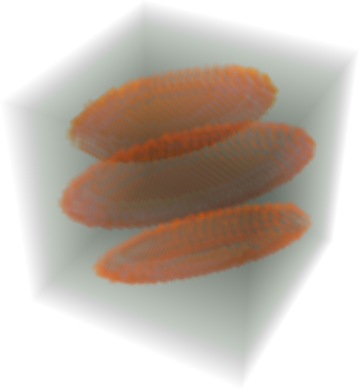
\includegraphics[width=1\linewidth]{images/disks_saliency}
	\end{minipage}~
	\begin{minipage}{.45\textwidth}
		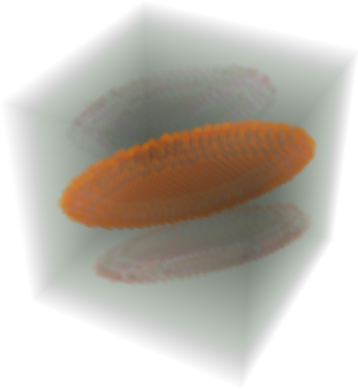
\includegraphics[width=1\linewidth]{images/disks_saliency_saturation}
	\end{minipage}
	\caption{The saliency fields computed from brightness (left) and saturation of voxels (right) respectively.}
	\label{fig:disks_saliency}
\end{figure}

\begin{figure}
	\centering
	\begin{minipage}{.45\textwidth}
		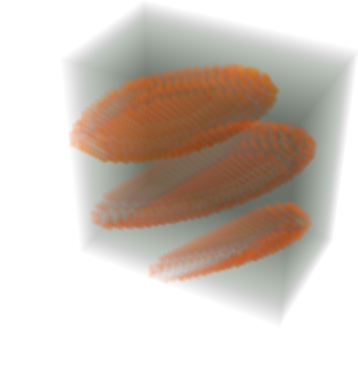
\includegraphics[width=1\linewidth]{images/disks_saliency_half}
	\end{minipage}~
	\begin{minipage}{.45\textwidth}
		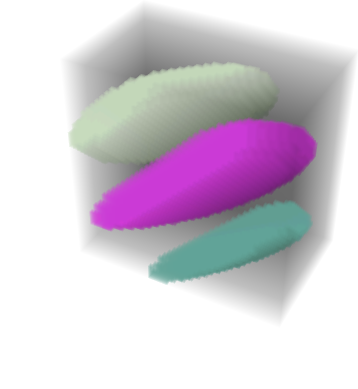
\includegraphics[width=1\linewidth]{images/disks_half}
	\end{minipage}
	\caption{The saliency fields emphasize the center and de-emphasize the surroundings of voxels. As in the clipped views of the saliency field (left) and the volume data set (right), the three solid disks are represented as hollow shapes in the saliency field.}
	\label{fig:disks_saliency_half}
\end{figure}

\subsection{Visibility-Weighted Saliency Fields of Features \label{visibility_weighted_saliency}}
The visibility field indicates the contribution of voxels, which is how much each voxel contributes to the final image, and the saliency field indicates the conspicuity of voxels, which is how much each voxel stands out from its surroundings.
The conspicuity in a 3D volume is similar to that in a 2D image and can be measured by the difference of visible properties between each location (voxel) and its surroundings \cite{duan_visual_2011}.
It would be desirable to have an indicator that represents both the contribution and conspicuity of the voxels.
Therefore, we propose a visibility-weighted saliency field, by weighting the saliency of voxels by their visibility, given the volume is rendered with a transfer function from a specific viewpoint.
The visibility-weighted saliency for voxel $ i $ is
\[ s_{i}(O,i,\sigma)= v_{i} L(O,i,\sigma)
\addtag \]
Hence we define $ S $ as the visibility-weighted saliency field of the volume $ V $.
\[ S=\set{s_{i}(O,i,\sigma)|i \in V} 
\addtag \]
Therefore, we define visibility-weighted saliency field of a feature $ F $ in the volume $ V $ ($ F\subseteq V $) as.
\[ S_{F}=\set{s_{i}(O,i,\sigma)|i \in F} 
\addtag \]

Then we define visibility-weighted saliency of feature $ F $ as
\[ W_{F}(O,i,\sigma)=\frac{\sum_{i \in F}{s_{i}(O,i,\sigma)}}{\sum_{i \in V}{s_{i}(O,i,\sigma)}} 
\addtag \]
Since $ F $ is a subset of $ V $, $ W_{F}(O,i,\sigma) $ must be in the interval $ [0,1] $.
$ S_{F} $ can be used as a score to indicate the saliency of feature $ F $ in terms of the appearance attribute $ O $.

Features can be defined by user-specified transfer functions or segmentation of the volume data.
Figure~\ref{fig:disks_visibility_saliency_fields} illustrates the visibility-weighted saliency fields of the three disk-like features.

\subsection{Visibility-Weighted Feature Saliency Histograms \label{weighted_feature_saliency}}
As mentioned in Section~\ref{saliency_fields}, the saliency field can be computed from different appearance attributes.
Multiple saliency fields computed from different appearance attributes can be combined together in order to represent different aspects of the visual saliency of voxels.
In our implementation, we use brightness and saturation respectively to compute visibility-weighted saliency fields and define the weighted sum of the two sets of feature saliency as visibility-weighted feature saliency.

%Similar to the visibility-weighted saliency in the previous section, the visibility-weighted saliency from brightness for voxel $ i $ is
%$ W_{F}(O_{b},i,\sigma) $ $ W_{F}(O_{s},i,\sigma) $
%\[ s_{i}(O_{s},i,\sigma)= v_{i} L(O_{b},i,\sigma)\]
%and the visibility-weighted saliency from saturation for voxel $ i $ is
%\[ s_{i}(O_{s},i,\sigma)= v_{i} L(O_{s},i,\sigma)\]
%Then we define the mean feature saliency as mean of the visibility-weighted saliency values computed using brightness and saturation respectively

\[ W_{F}=u_{1}W_{F}(O_{b},i,\sigma)+u_{2}W_{F}(O_{s},i,\sigma)
\addtag \]
where $ u_{1}$ and $ u_{2}$ are weights of different appearance attributes. $ u_{1}$ and $ u_{2}$ are both in the interval $[0,1] $ and $ u_{1}+u_{2}=1 $. $ W_{F}(O_{b},i,\sigma) $ is the visibility-weighted saliency of feature $ F $ computed using brightness of voxels and similarly $ W_{F}(O_{s},i,\sigma) $ is the visibility-weighted saliency of feature $ F $ from saturation of voxels.

Figure~\ref{fig:disks_saliency_chart_left} and Figure~\ref{fig:disks_saliency_chart_right} display bar charts of our visibility-weighted saliency of the three features and the feature visibility by Wang et al. \cite{wang_efficient_2011} for comparison.
We compute the saliency fields using brightness and saturation respectively and thus acquire two sets of feature saliency of the three features in the synthetic data set.
In Figure~\ref{fig:disks_saliency_chart_left} and Figure~\ref{fig:disks_saliency_chart_right}, the feature saliency from brightness shows similar patterns as the feature visibility. However, the feature saliency from saturation gives the highest score to the middle disk (magenta color), which indicates the middle disk is significantly more salient than the other two (light green and dark green) in terms of saturation. The visibility-weighted feature saliency combines the feature saliency from brightness and saturation with user-specified weights. 
%which combines the saliency fields derived from brightness and saturation of voxels.
The visibility-weighted feature saliency can be used as a measure to indicate the saliency of features in volume rendered images.
%The weights of different appearance attributes may be adjusted according to the user's need in specific tasks.
Equal weights of appearance attributes are assumed for now in our implementation, however, more detailed perceptual studies may determine more ideal weights.

\begin{figure}
	\centering
	\begin{minipage}{.3\textwidth}
		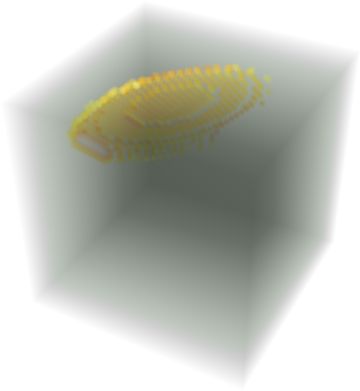
\includegraphics[width=1\linewidth]{images/disks_visibility_saliency_feature1_left}
	\end{minipage}~
	\begin{minipage}{.3\textwidth}
		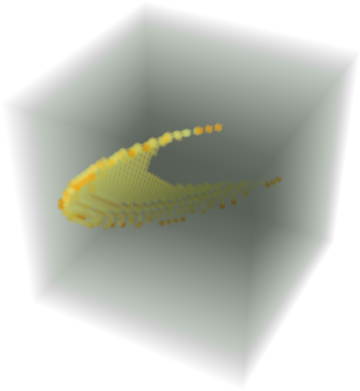
\includegraphics[width=1\linewidth]{images/disks_visibility_saliency_feature2_left}
	\end{minipage}~
	\begin{minipage}{.3\textwidth}
		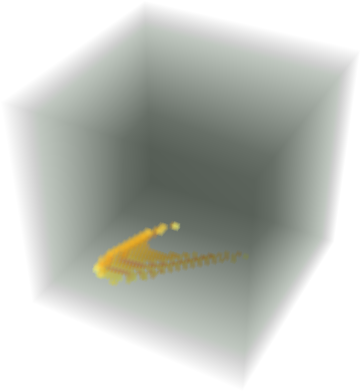
\includegraphics[width=1\linewidth]{images/disks_visibility_saliency_feature3_left}
	\end{minipage}
	\begin{minipage}{.3\textwidth}
		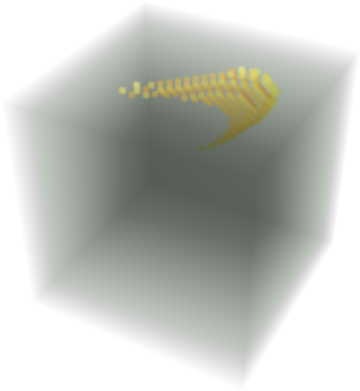
\includegraphics[width=1\linewidth]{images/disks_visibility_saliency_feature1_right}
	\end{minipage}~
	\begin{minipage}{.3\textwidth}
		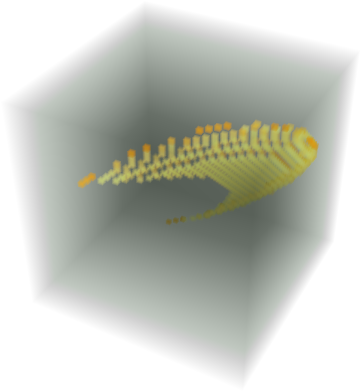
\includegraphics[width=1\linewidth]{images/disks_visibility_saliency_feature2_right}
	\end{minipage}~
	\begin{minipage}{.3\textwidth}
		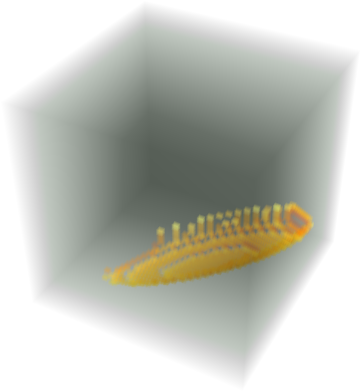
\includegraphics[width=1\linewidth]{images/disks_visibility_saliency_feature3_right}
	\end{minipage}
	\caption{Visibility-weighted saliency fields of the three disks. The first column shows the saliency fields of the top disk in the two viewpoints in Figure~\ref{fig:disks_combined}. The second and the third columns show the saliency fields for the middle disk and the bottom disk in the two viewpoints respectively.}
	\label{fig:disks_visibility_saliency_fields}
\end{figure}

\begin{figure}
	\centering
	\begin{minipage}{.45\textwidth}
		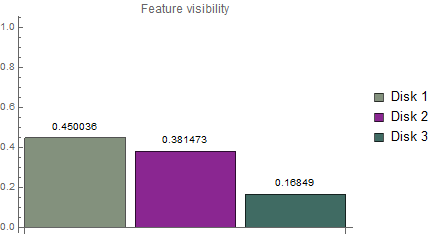
\includegraphics[width=1\linewidth]{images/disk_visibility_chart_left.png}
		\subcaption{}
	\end{minipage}~
	\begin{minipage}{.45\textwidth}
		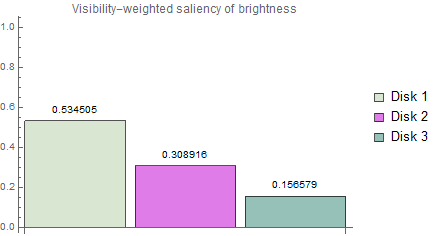
\includegraphics[width=1\linewidth]{images/disk_visibility_saliency_brightness_chart_left.png}
		\subcaption{}
	\end{minipage}
	\begin{minipage}{.45\textwidth}
		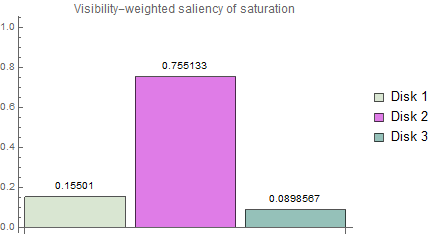
\includegraphics[width=1\linewidth]{images/disk_visibility_saliency_saturation_chart_left.png}
		\subcaption{}
	\end{minipage}~
	\begin{minipage}{.45\textwidth}
		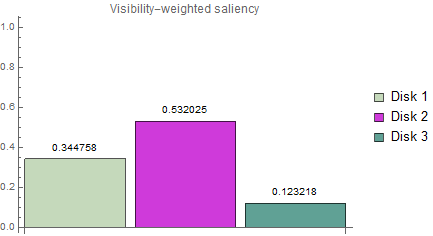
\includegraphics[width=1\linewidth]{images/disk_visibility_saliency_weighted_chart_left.png}
		\subcaption{}
	\end{minipage}
	\caption{The feature visibility \cite{wang_efficient_2011} histogram at top-left shows the sum of visibility values of all the voxels belonging to each feature.
		The two histograms of visibility-weighted feature saliency based brightness and saturation respectively (at top-right and at bottom-left) show the sum of visibility-weighted saliency of all the voxels belonging to each feature ($ W_{F}(O,i,\sigma) $ in Section~\ref{visibility_weighted_saliency}).
		The histogram of visibility-weighted feature saliency (at bottom-right) shows the visibility-weighted feature saliency with equal weights of brightness and saturation ($ W_{F} $ in Section~\ref{weighted_feature_saliency}).
		Feature visibility (top-left) and visibility-weighted feature saliency from brightness (top-right) both suggest that the top disk is the most visible and the bottom disk is the least visible.
		However, the middle disk with magenta color is significantly more salient than the other two disks (light green and dark green) in terms of saturation (the histogram at bottom-left).
	}
	\label{fig:disks_saliency_chart_left}
\end{figure}

\begin{figure}
	\centering
	\begin{minipage}{.45\textwidth}
		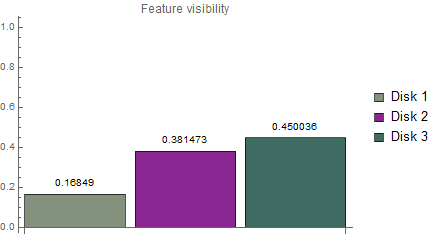
\includegraphics[width=1\linewidth]{images/disk_visibility_chart_right.png}
		\subcaption{}
	\end{minipage}~
	\begin{minipage}{.45\textwidth}
		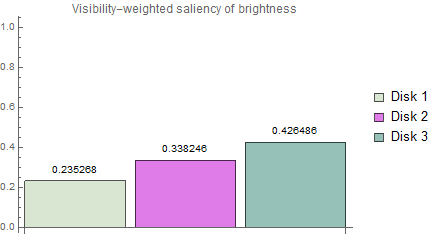
\includegraphics[width=1\linewidth]{images/disk_visibility_saliency_brightness_chart_right.png}
		\subcaption{}
	\end{minipage}
	\begin{minipage}{.45\textwidth}
		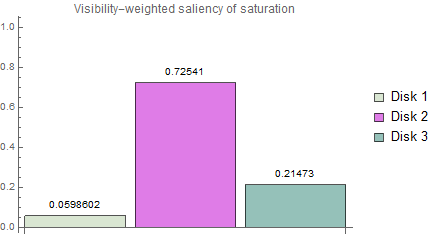
\includegraphics[width=1\linewidth]{images/disk_visibility_saliency_saturation_chart_right.png}
		\subcaption{}
	\end{minipage}~
	\begin{minipage}{.45\textwidth}
		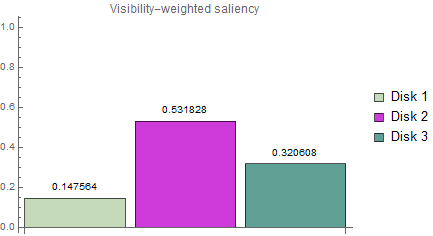
\includegraphics[width=1\linewidth]{images/disk_visibility_saliency_weighted_chart_right.png}
		\subcaption{}
	\end{minipage}
	\caption{Similar to Figure~\ref{fig:disks_saliency_chart_left}, in the viewpoint on the right in Figure~\ref{fig:disks_combined}, the bottom disk is the most visible according to feature visibility (histogram at top-left) and most salient according to feature saliency from brightness (histogram at top-right). However, feature saliency from saturation (histogram at bottom-left) suggests that the middle disk (magenta color) is significantly more salient than the other two (light green and dark green) in terms of saturation. The histogram at bottom-right is the visibility-weighted feature saliency with equal weights of brightness and saturation.}
	\label{fig:disks_saliency_chart_right}
\end{figure}

%\begin{figure}
%\centering
%\begin{minipage}{.22\textwidth}
%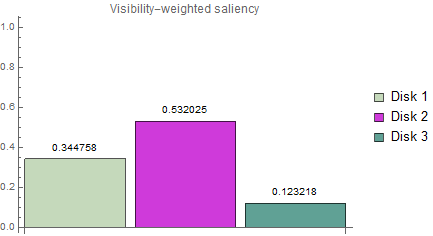
\includegraphics[width=1\linewidth]{images/disk_visibility_saliency_weighted_chart_left.png}
%\end{minipage}~
%\begin{minipage}{.22\textwidth}
%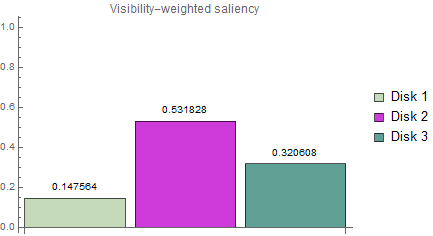
\includegraphics[width=1\linewidth]{images/disk_visibility_saliency_weighted_chart_right.png}
%\end{minipage}
%\caption{Weighted feature saliency of the three features in the left and the right viewpoint in Figure~\ref{fig:disks_combined}. The left bar chart is the mean of the middle and the right bar charts in Figure~\ref{fig:disks_saliency_chart_left} and the right bar chart is the mean of those two in Figure~\ref{fig:disks_saliency_chart_right}.}
%\label{fig:disks_mean_saliency_chart}
%\end{figure}

%-------------------------------------------------------------------------
\section{Use Case: Measuring Feature Saliency Resulting from Different Transfer Functions}
In this section, we present results of using our approach to measure visual saliency of features of a volume data set with two different transfer functions.

A tooth data set \cite{website:Roettger_volume_2013} is rendered with two different transfer functions to demonstrate the effectiveness of our approach. The first transfer function (Figure~\ref{fig:tooth}) assigns equal opacity to the three features.
The second transfer function (Figure~\ref{fig:tooth_2}) is designed to emphasize the enamel (the yellow material), thus it assigns high opacity the enamel and low opacity to the other two features (cementum \& pulp chamber and dentine).

By observation, it is clear that the transfer function in Figure~\ref{fig:tooth_2} is better in terms of visualizing the enamel than Figure~\ref{fig:tooth}. The purpose of our approach is to provide an automated objective measure to make this comparison. This is demonstrated through the output of the visibility-weighted salience fields of the two transfer functions (Figure~\ref{fig:tooth_saliency_field} and Figure~\ref{fig:tooth_saliency_field_2}).

In the visibility-weighted saliency fields of the first transfer function (Figure~\ref{fig:tooth_saliency_field}), all three features are reasonably salient.
%The visibility-weighted saliency fields display the contribution of three features to the volume rendered image respectively. In Figure~\ref{fig:tooth}, the material outside occludes the enamel inside, this can be seen from the visibility-weighted saliency fields in Figure~\ref{fig:tooth_saliency_field}.
%On the other hand, in Figure~\ref{fig:tooth_2},
% the two outer features have low opacity and the enamel inside has high opacity.
On the other hand, the visibility-weighted saliency fields of the second transfer function (Figure~\ref{fig:tooth_saliency_field_2}) suggest the enamel has significantly higher visual saliency in the volume rendered image.
%On the other hand, in Figure~\ref{fig:tooth_2}
The feature visibility and visibility-weighted feature saliency in Figure~\ref{fig:tooth_saliency_chart} and Figure~\ref{fig:tooth_saliency_chart_2} summarize the visibility and visual saliency of the three features specified by the transfer functions.

\begin{figure}
	\centering
	\begin{minipage}{.6\textwidth}
		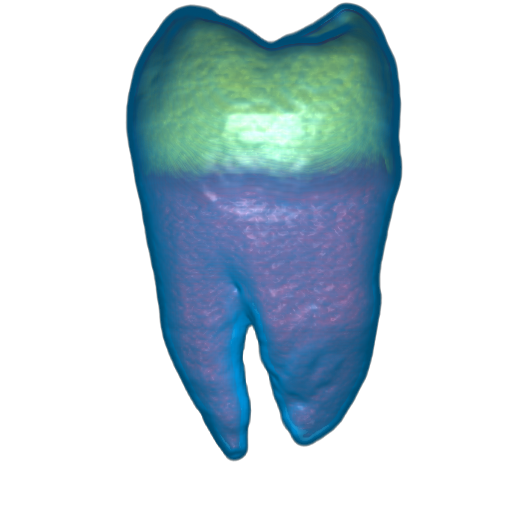
\includegraphics[width=1\linewidth]{images/tooth_naive.png}
	\end{minipage}~
	\begin{minipage}{.3\textwidth}
		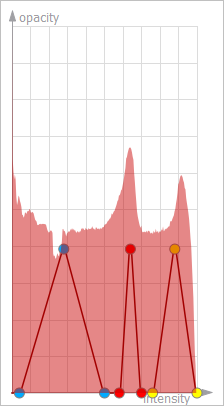
\includegraphics[width=1\linewidth]{images/tooth_tf.png}
	\end{minipage}
	\caption{A tooth data set with a transfer function revealing three features: cementum \& pulp chamber (blue), dentine (red) and enamel (yellow). Equal opacity is assigned to the three features in the transfer function.}
	\label{fig:tooth}
\end{figure}

\begin{figure}
	\centering
	\begin{minipage}{.3\textwidth}
		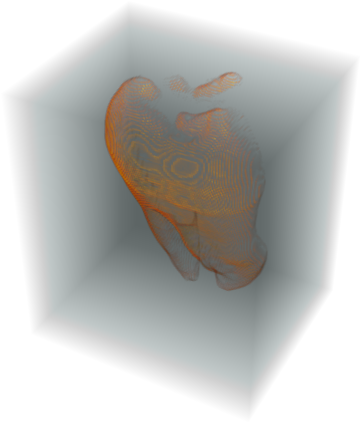
\includegraphics[width=1\linewidth]{images/tooth_visibility_saliency_feature1.png}
	\end{minipage}~
	\begin{minipage}{.3\textwidth}
		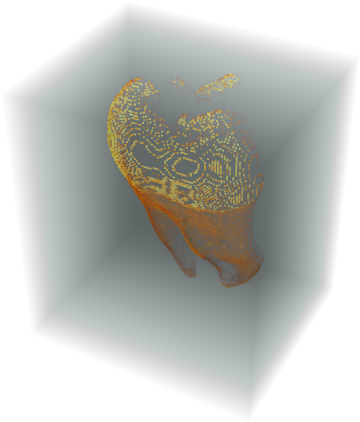
\includegraphics[width=1\linewidth]{images/tooth_visibility_saliency_feature2.png}
	\end{minipage}~
	\begin{minipage}{.3\textwidth}
		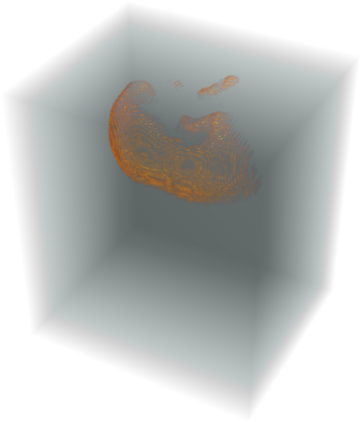
\includegraphics[width=1\linewidth]{images/tooth_visibility_saliency_feature3.png}
	\end{minipage}
	\caption{Visibility-weighted saliency fields of the three features, computed with the transfer function in Figure~\ref{fig:tooth}. From left to right, the features are cementum \& pulp chamber, dentine and enamel.}
	\label{fig:tooth_saliency_field}
\end{figure}

\begin{figure}
	\centering
	\begin{minipage}{.45\textwidth}
		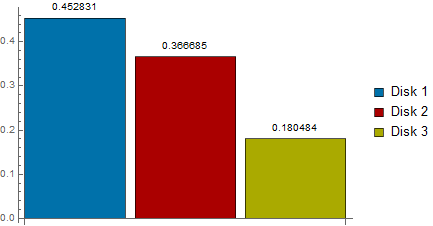
\includegraphics[width=1\linewidth]{images/tooth_visibility_chart.png}
	\end{minipage}~
	%\begin{minipage}{.2\textwidth}
	%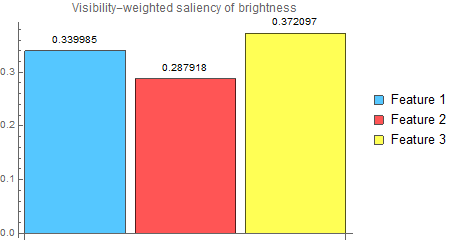
\includegraphics[width=1\linewidth]{images/tooth_visibility_saliency_brightness_chart.png}
	%\end{minipage}
	%\begin{minipage}{.2\textwidth}
	%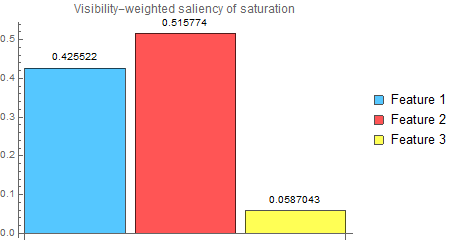
\includegraphics[width=1\linewidth]{images/tooth_visibility_saliency_saturation_chart.png}
	%\end{minipage}~
	\begin{minipage}{.45\textwidth}
		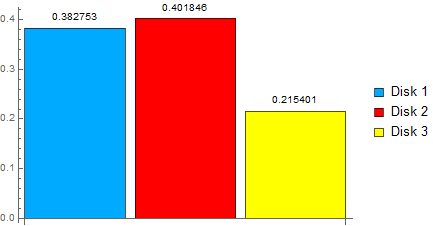
\includegraphics[width=1\linewidth]{images/tooth_visibility_saliency_weighted_chart.png}
	\end{minipage}
	\caption{Feature visibility \cite{wang_efficient_2011} (darker histogram on the left) and visibility-weighted saliency (brighter histogram on the right) of the three features, computed with the transfer function in Figure~\ref{fig:tooth}.}
	\label{fig:tooth_saliency_chart}
\end{figure}

\begin{figure}
	\centering
	\begin{minipage}{.6\textwidth}
		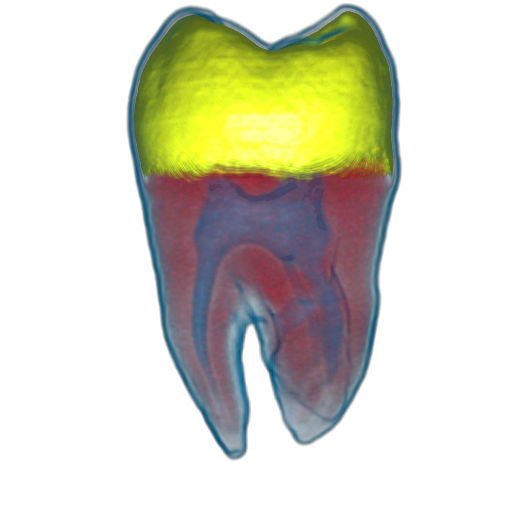
\includegraphics[width=1\linewidth]{images/tooth_balance_gpu.png}
	\end{minipage}~
	\begin{minipage}{.3\textwidth}
		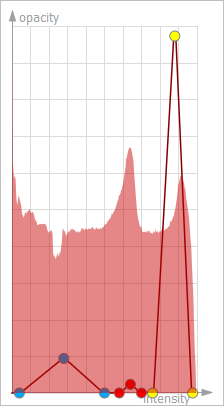
\includegraphics[width=1\linewidth]{images/tooth_balance_tf.png}
	\end{minipage}
	\caption{A tooth data set with a transfer function particularly highlighting the enamel (yellow)}
	\label{fig:tooth_2}
\end{figure}

\begin{figure}
	\centering
	\begin{minipage}{.3\textwidth}
		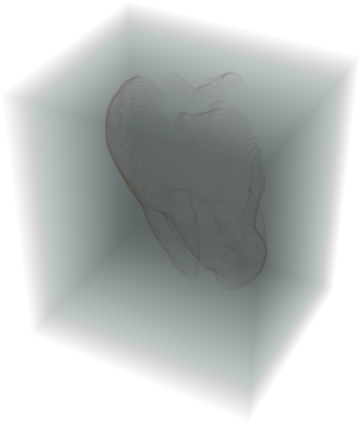
\includegraphics[width=1\linewidth]{images/tooth_2_visibility_saliency_feature1.png}
	\end{minipage}~
	\begin{minipage}{.3\textwidth}
		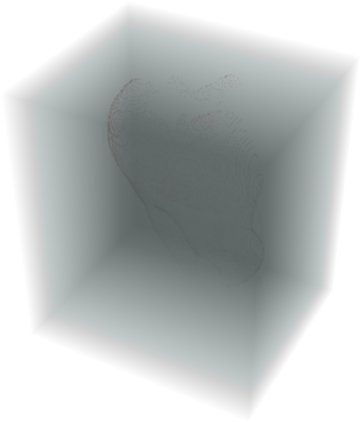
\includegraphics[width=1\linewidth]{images/tooth_2_visibility_saliency_feature2.png}
	\end{minipage}~
	\begin{minipage}{.3\textwidth}
		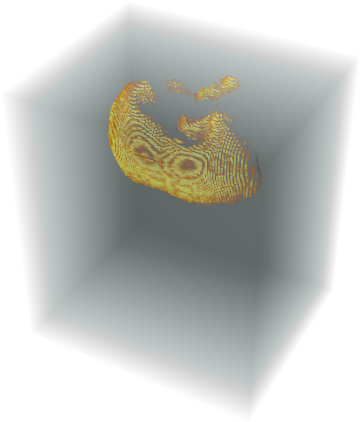
\includegraphics[width=1\linewidth]{images/tooth_2_visibility_saliency_feature3.png}
	\end{minipage}
	\caption{Visibility-weighted saliency field of the three features, computed with the transfer function in Figure~\ref{fig:tooth_2}. From left to right, the features are cementum \& pulp chamber, dentine and enamel.}
	\label{fig:tooth_saliency_field_2}
\end{figure}

\begin{figure}
	\centering
	\begin{minipage}{.45\textwidth}
		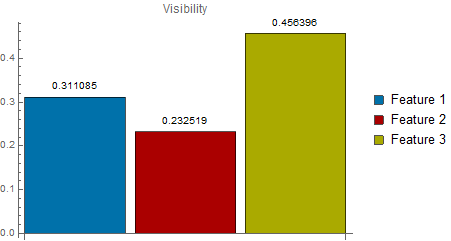
\includegraphics[width=1\linewidth]{images/tooth_2_visibility_chart.png}
	\end{minipage}~
	%\begin{minipage}{.2\textwidth}
	%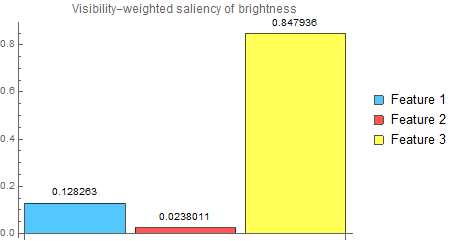
\includegraphics[width=1\linewidth]{images/tooth_2_visibility_saliency_brightness_chart.png}
	%\end{minipage}
	%\begin{minipage}{.2\textwidth}
	%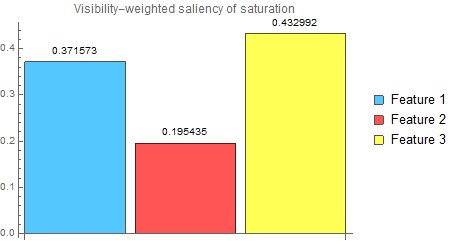
\includegraphics[width=1\linewidth]{images/tooth_2_visibility_saliency_saturation_chart.png}
	%\end{minipage}~
	\begin{minipage}{.45\textwidth}
		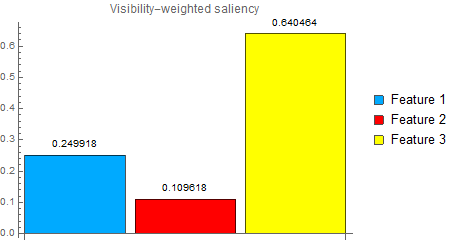
\includegraphics[width=1\linewidth]{images/tooth_2_visibility_saliency_weighted_chart.png}
	\end{minipage}
	\caption{Feature visibility (darker histogram on the left) and visibility-weighted feature saliency (brighter histogram on the right) of the three features, computed with the transfer function in Figure~\ref{fig:tooth_2}.}
	\label{fig:tooth_saliency_chart_2}
\end{figure}

%-------------------------------------------------------------------------
\section{Experiment \label{experiment_section}}
%An experiment was performed to investigate how each style, described in Section 5.3.2,
%affected a user’s ability to determine the shape of the target isosurface. The primary aim
%of the visualisations is to use all volumetric data to give a clear impression of a certain
%part of each dataset while showing the rest of the object data for reference. For this reason
%it was necessary to test how well each style represented each dataset, which meant a shape
%perception experiment was the most suitable test and it was chosen over task-based or
%eye-tracking experiments. We hypothesised that by adding edges and abstractions to the
%dataset, the target isosurface level would be clearer to the user and the background volume
%would be de-emphasised, therefore increasing a user’s understanding of the dataset.
%To test a user’s perception of shape, an experiment was run that involved placement
%of gauges on static images. This protocol was described in previous experiments such

An experiment was performed to investigate how the visual saliency of objects in volume visualization was perceived by human users. A typical objective in volume visualization is to provide a clear impression of a certain part (i.e. a feature) of a volume data set while showing the rest of the data set for reference \cite{redmond_influencing_2010}.
For this reason, it is necessary to test how well the shapes of features are perceived by human users.
The aim of this experiment is to gather subjective opinion scores regarding how clear and distinct the features are in the images shown to the participants, and then compare the user opinion scores against the proposed computational visual saliency metric.

%To judge the effectiveness of the proposed approach, a human study was conducted to construct a subjective data set for assessing visual saliency of features in volume visualization as perceived by human users.
%The aim of this experiments is to gather human rating of visual saliency data in order to evaluate the proposed computational visual saliency metric for volume visualization.

\subsection{Source Images and Participants}
%This section describes the human study and experiments performed using it.
The volume rendering images used for the study were rendered by Voreen \cite{meyer-spradow_voreen:_2009} with a variety of transfer functions highlighting different features from various viewpoints. The volume data sets used in the experiment are publicly available on the Internet.
8 volume data sets were used to produce images for the experiment and the images of 2 data sets (CThead and lobster) were only used in the training session at the beginning of the experiment.
The results of 6 volume data sets were analyzed. These data sets are engine block, foot, MRbrain, nucleon, vismale, tooth and vismale
%and horse embryo 
\cite{website:Roettger_volume_2013} \cite{website:Voreen_datasets_2013}.
%There were 30 people participated in the experiment. Among the participants, there were 20 males and 10 females, all aged between 22 and 39 years old.
30 participants (20 male and 10 female) took part in the experiment. All were aged between 22 and 39 years old and consisted of postgraduates, undergraduates and researchers. Over half of the participants have computer science background. Only one participant reported that he had slight color blindness (red-green). This participant confirmed that he had no problem in distinguishing the colors of features in the experiment.

\subsection{Methods and Measurements}
In the experiment, participants would sit in front of a computer display viewing images generated from volume visualization. The experiment would investigate how participants perceive the visual saliency of different objects in the images. The participants' task would be to score the images on a scale of 1 to 5 by keyboard input.
In each trial, a screen indicating the feature of interest would be shown to the participant for 3 seconds, followed by a screen displaying a volume rendered image for 17 seconds.
The experiment would last approximately 20 minutes.
Some images were shown more than once in the experiment in order to detect whether the participants's scores are consistent during the experiment.

\subsection{2D Feature Saliency}
A widely used saliency model is the saliency map by Itti et al. \cite{itti_model_1998}.
The architecture and components of this model mimic the properties of primate early vision.
Three visual properties, i.e. intensity contrast, color opponency and orientation are considered in the model in order to determine whether an image pixel stands out from its surroundings.
The saliency map is a 2D image indicating the visual saliency of pixels in the input image. Although 2D saliency maps can not be directly used to estimate the visual saliency of 3D features, an inverse distance weighting \cite{shepard_two-dimensional_1968} can be applied to divide a 2D saliency map into several feature saliency maps, one for each feature (see Appendix~\ref{2d_saliency_map} for details). Subsequently, the visual saliency of each feature can be estimated with the total intensity of each 2D feature saliency map. 

\subsection{Data Analysis}
Since the opinion scores obtained from participants in the experiment may not be normally distributed or consistently applied across participants and data sets, this structure of data may violate the assumptions of some standard statistical tests \cite{cunningham_experimental_2011}.
%Spearman's rank correlation does not assume normality of the variables.
Because we are interested in the monotonic relationships between the variables, Spearman's rank correlation, which does not assume normality of the variables, would be suitable for evaluating the strength of monotonic associations of the observed scores (mean opinion scores) and scores calculated from computational metrics. 

We applied the Spearman's rank correlation to analyze the monotonic association between the mean opinion scores (MOS) and three computational metrics, i.e. our visibility-weighted saliency (VWS) metric, feature visibility (FV) based on \cite{wang_efficient_2011} and 2D feature saliency (2DFS).

As shown in Figure~\ref{fig:mos_vs_vws}, there are strong positive correlations between MOS and VWS ($ 0.66985 $), and MOS and FS ($ 0.677018 $) respectively. On the other hand, there is a moderate positive correlation between MOS and 2DFS ($ 0.550472 $). Both VWS and FS are more monotonic correlated to MOS than 2DFS, and FV is slightly better than VWS by about $ 0.007 $.

The p-values indicate statistical significance of the associations. In our results, the p-values for all the three cases are very small (below $2 \times 10^{-5} $). Therefore, we can reject the null hypothesis (there is no association between the variables) and conclude that there are associations between MOS and VWS, FS and 2DFS respectively.

In addition, we group MOS by features to provide a more detailed view of the correlation between MOS and VWS.
Figure~\ref{fig:mos_vs_metric} displays line plots of MOS versus VWS for each feature of the data sets separately, with the data points sorted by VWS on the x axis.
Because some images were shown more than once in the experiment, the resulting data points have the same VWS and very similar MOS in the line plots.
Although the line plots are not strictly monotonic (i.e. MOS and VWS are not strictly monotonically correlated), we notice that they have loose monotonic associations.

The analysis of the experiment results indicates that our VWS is better than 2DFS and equivalent to FV in terms of predicting human perception of visual saliency in volume rendering images.

\begin{figure}
	\centering
	\begin{minipage}{.33\textwidth}
		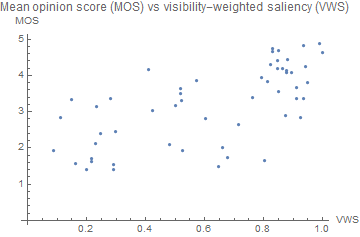
\includegraphics[width=1\linewidth]{images/mos_vs_vws.png}
		\subcaption{ Spearman's $\rho=0.66985 $, P-value$=3.03794 \times 10^{-8} $ }
	\end{minipage}~
	\begin{minipage}{.33\textwidth}
		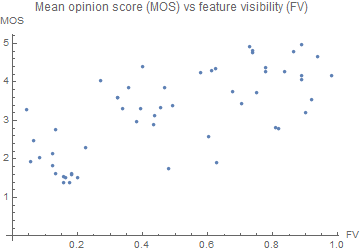
\includegraphics[width=1\linewidth]{images/mos_vs_visibility}
		\subcaption{ Spearman's $\rho=0.677018 $, P-value$=1.90023 \times 10^{-8} $ }
	\end{minipage}~
	\begin{minipage}{.33\textwidth}
		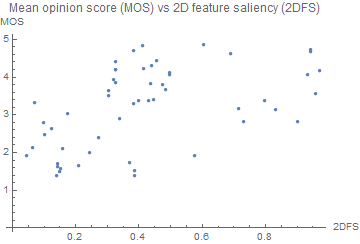
\includegraphics[width=1\linewidth]{images/mos_vs_2dfs}
		\subcaption{ Spearman's $\rho=0.550472 $, P-value$=1.61418 \times 10^{-5} $ }
	\end{minipage}
	\caption{Spearman's rank correlation of 54 opinion scores against the corresponding visibility-weighted saliency (VWS), feature visibility (FV) and 2D feature saliency (2DFS) respectively. There are strong positive correlations between MOS and VWS (a) and between MOS and FV (b). There is a moderate positive correlation between MOS and 2DFS (c).}
	\label{fig:mos_vs_vws}
\end{figure}

\begin{figure}
	\centering
	\begin{minipage}{.24\textwidth}
		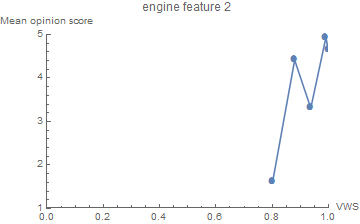
\includegraphics[width=1\linewidth]{images/mos_vs_metric_engine_feature_2}
		\subcaption{}
	\end{minipage}~
	\begin{minipage}{.24\textwidth}
		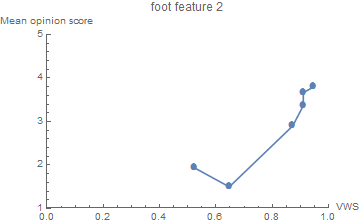
\includegraphics[width=1\linewidth]{images/mos_vs_metric_foot_feature_2}
		\subcaption{}
	\end{minipage}~
%	\begin{minipage}{.24\textwidth}
%		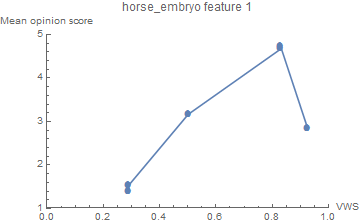
\includegraphics[width=1\linewidth]{images/mos_vs_metric_horse_embryo_feature_1}
%		\subcaption{}
%	\end{minipage}~
	\begin{minipage}{.24\textwidth}
		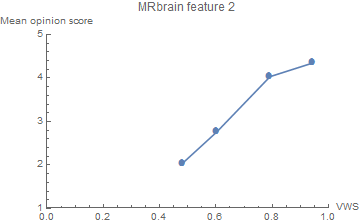
\includegraphics[width=1\linewidth]{images/mos_vs_metric_MRbrain_feature_2}
		\subcaption{}
	\end{minipage}~
	\begin{minipage}{.24\textwidth}
		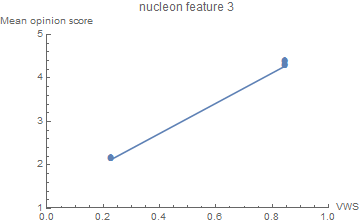
\includegraphics[width=1\linewidth]{images/mos_vs_metric_nucleon_feature_3}
		\subcaption{}
	\end{minipage}
	\begin{minipage}{.24\textwidth}
		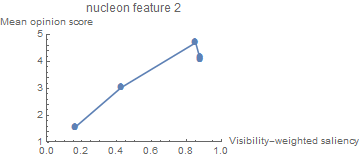
\includegraphics[width=1\linewidth]{images/mos_vs_metric_nucleon_feature_2}
		\subcaption{}
	\end{minipage}~
	\begin{minipage}{.24\textwidth}
		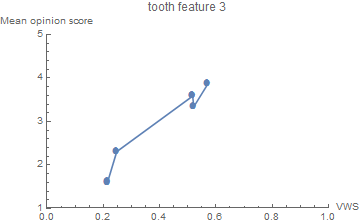
\includegraphics[width=1\linewidth]{images/mos_vs_metric_tooth_feature_3}
		\subcaption{}
	\end{minipage}~
	\begin{minipage}{.24\textwidth}
		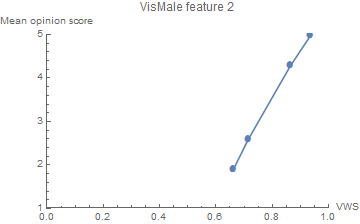
\includegraphics[width=1\linewidth]{images/mos_vs_metric_vismale_feature_2}
		\subcaption{}
	\end{minipage}~
	\begin{minipage}{.24\textwidth}
		\includegraphics[width=1\linewidth]{images/mos_vs_metric_vismale_feature_1}
		\subcaption{}
	\end{minipage}
	\caption{Line plots of MOS versus VWS for each feature of the data sets separately}
	\label{fig:mos_vs_metric}
\end{figure}

\subsection{Varying Saturation and Brightness in Transfer Functions}
A major difference between our visibility-weighted saliency and the feature visibility is that our approach reflects two aspects of the resulting visualization, i.e. voxel visibility and visual saliency, while the feature visibility only reflects voxel visibility.
Figure~\ref{fig:tooth_naive_optimized_linesearch} displays an image of the tooth data set and its feature visibility and visibility-weighted saliency.
In Figure~\ref{fig:tooth_naive_optimized_linesearch_red} and Figure~\ref{fig:tooth_naive_optimized_linesearch_yellow}, the saturation and brightness of the red feature and the yellow feature are reduced respectively. As shown in the two figures, our approach reflects the change of saturation and brightness of volume visualization.

\begin{figure}
	\centering
	\begin{minipage}{.24\textwidth}
		\includegraphics[width=1\linewidth]{images/tooth_naive_optimized_linesearch}
		\subcaption{}
	\end{minipage}~
	\begin{minipage}{.24\textwidth}
		\includegraphics[width=1\linewidth]{images/tooth_naive_optimized_linesearch_visibility_chart}
		\subcaption{}
	\end{minipage}~
	\begin{minipage}{.24\textwidth}
		\includegraphics[width=1\linewidth]{images/tooth_naive_optimized_linesearch_visibility_saliency_weighted_chart}
		\subcaption{}
	\end{minipage}
	\caption{(a) The tooth data set; (b) Feature visibility; (c) Visibility-weighted saliency}
	\label{fig:tooth_naive_optimized_linesearch}
\end{figure}

\begin{figure}
	\centering
	\begin{minipage}{.24\textwidth}
		\includegraphics[width=1\linewidth]{images/tooth_naive_optimized_linesearch_red_low_saturation}
		\subcaption{}
	\end{minipage}~
	\begin{minipage}{.24\textwidth}
		\includegraphics[width=1\linewidth]{images/tooth_naive_optimized_linesearch_red_low_saturation_visibility_saliency_weighted_chart}
		\subcaption{}
	\end{minipage}~
	\begin{minipage}{.24\textwidth}
		\includegraphics[width=1\linewidth]{images/tooth_naive_optimized_linesearch_red_low_brightness}
		\subcaption{}
	\end{minipage}~
	\begin{minipage}{.24\textwidth}
		\includegraphics[width=1\linewidth]{images/tooth_naive_optimized_linesearch_red_low_brightness_visibility_saliency_weighted_chart}
		\subcaption{}
	\end{minipage}
	\caption{(a) Low saturation for the red feature; (b) The visibility-weighted saliency of (a); (c) Low brightness for the red feature; (d) The visibility-weighted saliency of (c)}
	\label{fig:tooth_naive_optimized_linesearch_red}
\end{figure}

\begin{figure}
	\centering
	\begin{minipage}{.24\textwidth}
		\includegraphics[width=1\linewidth]{images/tooth_naive_optimized_linesearch_yellow_low_saturation}
		\subcaption{}
	\end{minipage}~
	\begin{minipage}{.24\textwidth}
		\includegraphics[width=1\linewidth]{images/tooth_naive_optimized_linesearch_yellow_low_saturation_visibility_saliency_weighted_chart}
		\subcaption{}
	\end{minipage}~
	\begin{minipage}{.24\textwidth}
		\includegraphics[width=1\linewidth]{images/tooth_naive_optimized_linesearch_yellow_low_brightness}
		\subcaption{}
	\end{minipage}~
	\begin{minipage}{.24\textwidth}
		\includegraphics[width=1\linewidth]{images/tooth_naive_optimized_linesearch_yellow_low_brightness_visibility_saliency_weighted_chart}
		\subcaption{}
	\end{minipage}
	\caption{(a) Low saturation for the yellow feature; (b) The visibility-weighted saliency of (a); (c) Low brightness for the yellow feature; (d) The visibility-weighted saliency of (c)}
	\label{fig:tooth_naive_optimized_linesearch_yellow}
\end{figure}


%-------------------------------------------------------------------------
\section{Conclusions}
In this paper, we propose visibility-weighted saliency as an improved measure of the visual saliency of features in volume rendered images, in order to assist users in choosing suitable viewpoints and designing effective transfer functions to visualize the features of interest.
%The visibility-weighted saliency are presented in two different ways, i.e. visibility-weighted saliency fields and feature saliency histograms. Visibility-weighted saliency fields display the spatial distribution of visual saliency of features and feature saliency histograms provide quantitative information about the perceptual importance of the features.
With visibility-weighted saliency, the saliency of features rendered in different viewpoints with different transfer functions can be measured in a quantitative and fully automated way.
%In future work we plan to validate our work by conducting an eye-tracking-based user study. In addition, we would like to study other appearance attributes apart from brightness and saturation, and study the weighting between these attributes.
%-------------------------------------------------------------------------
